\documentclass[a4paper,11pt]{article}

\usepackage[plain]{fullpage} %Error.
\usepackage{graphicx}  %This enables the inclusion of pdf graphic files in figures
\usepackage{wrapfig}
\usepackage{array}
\usepackage[hidelinks]{hyperref}
\usepackage{color}
\definecolor{light-gray}{gray}{0.95}
\usepackage{listings}
\lstset{
basicstyle=\scriptsize, 
morecomment=[l]{/*},
backgroundcolor=\color{light-gray}, 
xleftmargin=.10in,
xrightmargin=.10in,
language=C
}

\title{\textbf{Report: Assignment 3}}
\author{Group 9: \O yvin Richardsen, Sandor Zeestraten, Stian Habbestad}
\date{{Norwegian University of Science and Technology \\
TDT4258 Energy Efficient Computer Design \\}
\today}
 
\begin{document}
\maketitle

\begin{abstract}
In this assignment we write C code for an AVR microcontroller on linux. Through this assignment we aim to become more familiar with C coding for AVR32, linux and how to write a driver for linux. Our approach was to first replicate the features of the previous assignment, then we ..................
\end{abstract}

\bigskip
\tableofcontents
\newpage

\section{Introduction}

In this exercise we write a game in C, which is executed on top of linux on a STK1000 development board. We have written a pair of drivers to handle leds and buttons...................

\section{Description and methodology}

\textbf{Forrige rapport: organize report better (overview and block diagram before description of code fragments and functions). Ergo, block diagram her?}\\

First off we started out with trying to install linux on the STK1000 development board. This turned out to be a tricky affair. We had a step by step guide for compiling linux that we followed, but with no luck. Luckily there was mentioned an image of a precompiled linux that we could extract to the SD card. After some mixing back and forth with environment variables from the other u-boot.bin file(from itslearning) into the one we were using we finally started to get somewhere. 

\textbf{(d e bare å korrigera osv) }

Once we had linux up and running we started out with a simple "Hello world" program to verify things were working. Now we started out with programming a driver for the LEDs. We sometimes thought we had found the solution, but we still hadn't figured it out correctly. We gave the LED driver a pause and started to communicate with the frame buffer in linux. 

First off we thought maybe this file had to be a kernel module as well, but we soon understood that we needed acceess to quite a few libraries to make the memory mapping work. We started with generating a random bit values for the display and went on with more logical values, for example a third of the screen was made red. As we tried to read bit values from an image of the file format bitmap, we started to see that there were some errors in regards to how we read the file. 

\emph{linux compiling, image to sd, previous assignment, driver(led and button), framebuffer, porting of sokoban to C, sound, generated sounds, }

\subsection{Game}
\begin{figure}[h]
\centering
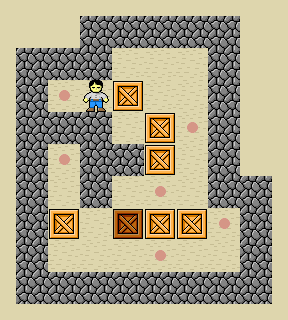
\includegraphics{images/sokoban.png}
\caption{An example implementation of Sokoban by Borgar Porsteinsson \cite{sokobanscreen}.}
\label{fig:sokobanimage}
\end{figure}

\subsubsection{Sokoban}
The game we chose to implement was a simple top-down puzzle game called \textit{Sokoban}\cite{sokoban}. The point of the game is for the player to push boxes onto marked goal squares. The levels are small maps confined by walls which cannot be walked through. The puzzle is solved when all the boxes are on the goal squares. We had some previous experience of implementing this game in Java in the course TDT4100: Object Oriented Programming. We therefore chose to port it to C.

\subsubsection{Levels}
The levels are defined by it's dimensions and an array of characters of the different elements. For more information see the level format page on Sokoban Wiki \cite{sokobanlevel}. See table \ref{tab:levelformat} for the level format we use.

\begin{table}[h]
\centering
\begin{tabular}{|l|l|}
\hline \textbf{Level element} & \textbf{Character} \\ 
\hline Wall & \# \\ 
\hline Player & @ \\ 
\hline Player on goal square & + \\ 
\hline Box & \$ \\ 
\hline Box on goal square & * \\ 
\hline Goal square & . \\ 
\hline Floor & (whitespace) \\ 
\hline 
\end{tabular}
\caption{The level format.}
\label{tab:levelformat}
\end{table}

The first level is defined below in figure \ref{fig:leveldef}. It is the simplest solvable level where the box just has to pushed to the left.
\begin{figure}[h]
\begin{lstlisting}
// From sokoban_leveldefs.h
#define level1dimX 5
#define level1dimY 3
char level1[] = "######@$.######";

// The level above looks like this when formatted.
#####
#@$.#
#####
\end{lstlisting}
\caption{Definition of the first level.}
\label{fig:leveldef}
\end{figure}

\subsubsection{Controls}
The game can 
\begin{table}[h]
\centering
\begin{tabular}{|l|l|}
\hline \textbf{Switch} & \textbf{Action} \\ 
\hline SW7 & Move left \\ 
\hline SW6 & Move down \\ 
\hline SW5 & Move up \\ 
\hline SW4 & Move right \\ 
\hline SW3 & Undo move \\ 
\hline SW2 & Redo move \\ 
\hline SW1 & Reset level \\ 
\hline SW0 & Display win screen \\ 
\hline 
\end{tabular}
\caption{Game controls} 
\label{tab:gamecontrols}
\end{table}

\subsubsection{Code}
\begin{lstlisting}
void button_isr(void) {
\end{lstlisting}

\begin{center}
\centering
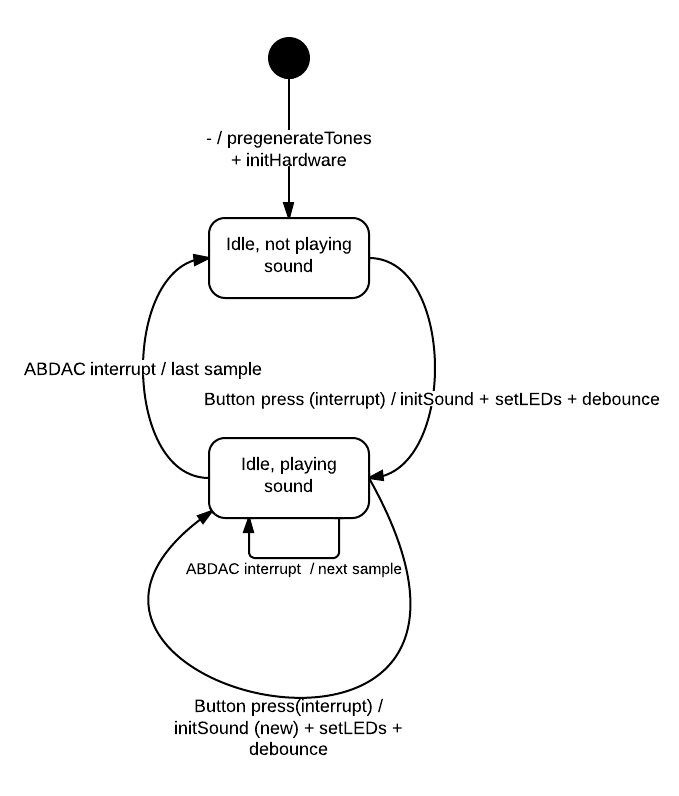
\includegraphics[scale=0.75]{images/lucid_chart.png}
\linebreak
Figure 1: State Diagram of the program
\end{center}

\newpage

\subsection*{Debugging}

%Here is a screenshot (Figure 2) showing us debugging our \emph{generateTriangle} function which generates triangle sound wave samples. More specifically we check that the values we get from each part of our (complex) mathematical expression are valid. 

\begin{center}

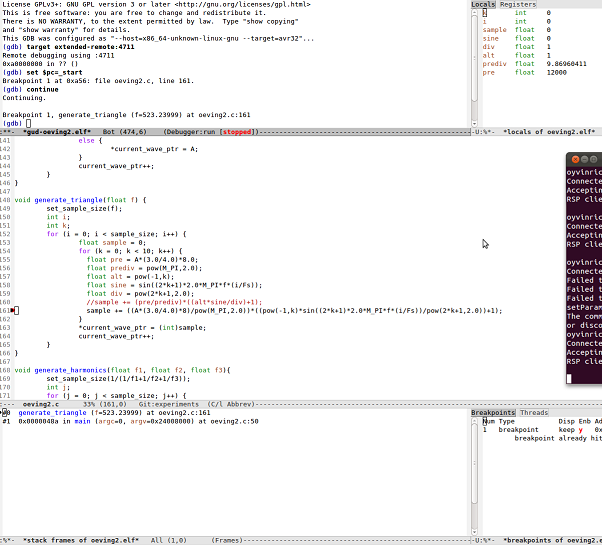
\includegraphics{images/debugsmall.png}
Figure 2: Debugging the \emph{generateTriangle} function
\end{center}

\section{Results}
This exercise resulted in a working sokoban game on the STK1000 development board displayed. The game is played by using the buttons as controllers to move around in the game which is displayed on the LCD screen. In addition to a general "arrow key" setup, there is also a possibility to undo and redo with the buttons. 

There are sounds and LEDs to help you understand the game play better through audiovisual feedback. The LEDs show how many crates you have left in the game, and when you win all LEDs will blink several times. There are sounds for the start of the game, when you place a crate on a target, when you remove a crate from a target, when you hit a wall and when you win. When you win there will also be a splash screen telling you that you've won. 

Technically the resulting game is written in C code on top of a linux operating system. To manage the LEDs and buttons we have written two correspondig linux drivers that operates as interfaces between the STK1000 development board and linux. 


\section{Tests}
\paragraph{Description}
%We've created a few test scenarios in order to test different cases of our code for playing sounds. The tests were conducted by a person interacting with the switches wearing a headset, and another person logging the results. The main equipment was the STK1000 development board, JTAGICE MKII and a headset. The jumpers of the board were set as specified in the compendium (section 3.4.1) \cite{komp}. The GPIO was connected as following: Port B to the LEDs and Port C to the switches.

\paragraph{Results}
%Below is a table of the different tests we ran, the preconditions and the results. We did not pass the \emph{Bouncing} test. Here we checked whether a sound would play without any interruptions during a switch press (both up and down). Releasing the button provides a new interrupt, which calls the button interrupt routine of our program, which further delays the waiting sound sample, causing a noticeable effect on the sound.

\begin{center}
\footnotesize
\renewcommand{\arraystretch}{1.25} %vertical cell padding
\begin{tabular}[pos]{|m{45pt}|m{80pt}|m{90pt}|m{105pt}|m{60pt}|}
\hline  \textbf{Name} & \textbf{Description} & \textbf{Conditions} & \textbf{Expected} & \textbf{Results} \\ 

\hline Steady-state test & Power is on and the main program is running & The board has been programmed and powered on & The board is powered and no LEDs or sounds should be on & Passed \\

\hline SFX1 & The first SFX plays & The main program is running & \emph{SFX1} plays once after \emph{SW7} is pressed. \emph{LED7} should be turned on & Passed \\

\hline SFX2 & The first SFX plays & The main program is running & \emph{SFX2} plays once after \emph{SW6} is pressed. \emph{LED6} should be turned on & Passed \\

\hline SFX3 & The first SFX plays & The main program is running & \emph{SFX3} plays once after \emph{SW5} is pressed. \emph{LED5} should be turned on & Passed \\ 

\hline Intro theme & The intro theme plays & The main program is running & The intro theme plays once after \emph{SW4} is pressed. \emph{LED4} should be turned on & Passed \\

\hline Bouncing & Any sound should only be played once per press of switch & Press down any switch from \emph{SW7} to \emph{SW4} and let it go & The sound should finish playing without any interruptions & Failed \\

\hline Change sound & Play a sound while another sound is already playing & A switch has been pressed and a sound is playing. While playing another switch has been pressed & The sound of the newly pressed switched should be playing & Passed \\ 

\hline Stop & Stop playing sounds when pressing any switch from \emph{SW3} to \emph{SW0} & Press any switch from \emph{SW3} to \emph{SW0} while sound is playing & The sound should stop playing & Passed \\ 

\hline 
\end{tabular} 
\end{center}

\newpage

\section{Evaluation of assignment}
This assignment was more demanding yet also more fun than the first assignment. The learning curve was a bit harder as not all of us had coded much in C before, but it was a nice opportunity to learn.

\section{Conclusion}
We learned how to generate and play different sounds in C. This will be helpful when we start coding the next assignment. In the end we have four different sounds. Three short sound effects and one melody. 

\footnotesize{  % This makes the Reference items print in footnotesize fonts
\begin{thebibliography}{N}

\bibitem[1]{avrdoc} AVR32 Architecture Document
\url{http://www.atmel.com/images/doc32000.pdf}

\bibitem[2]{stkdoc} AT32AP7000 Datasheet
\url{http://www.atmel.com/Images/doc32003.pdf}

\bibitem[3]{komp} TDT4258 Compendium
\url{http://www.idi.ntnu.no/emner/tdt4258/_media/kompendium.pdf}

\bibitem[4]{sokoban} Description of the game Sokoban on Sokoban Wiki . Retrieved 23.04.13.
\url{http://www.sokobano.de/wiki/index.php?title=The_rules_of_the_game}

\bibitem[5]{sokobanlevel} Description of Sokobon levels on Sokoban Wiki. Retrieved 23.04.13.
\url{http://www.sokobano.de/wiki/index.php?title=Level_format}

\bibitem[5]{sokobanscreen} Screenshot based on Sokoban skins on GitHub. Retrieved 23.04.13.
\url{https://github.com/borgar/sokoban-skins}


\end{thebibliography}  
}

\end{document} 
